\section{Model Ablations}\label{sec:model_ablations}
To contextualise the performance of \texttt{gpt-oss-120b}, we ran \name{} with four additional frontier LRMs, conducting ground-truth evaluations for each stage. We find variation in performance across stages with no clear best model (\cref{fig:model_ablation}). \texttt{Kimi-K2.5} and \texttt{gpt-oss-120b} perform best at the article screening stages, with the former excelling in title \& abstract screening ($F_1 = 0.77$) and the latter in full-text screening($F_1 = 0.63$). All models struggle with parameter extraction, with the highest performance again achieved by \texttt{Kimi-K2.5} ($F_1 = 0.87$). \texttt{GLM-4.7} performs well specifically for extracting models, while \texttt{GPT-5.2} stands out when extracting outbreaks. \texttt{DeepSeek-V3.2} exhibits the most variable performance across stages. It is the worst-performing model by some margin during article screening, but becomes competitive during the extraction phase where it is enabled with function calling, most evidently in model and outbreak extraction.

The smallest model by size, \texttt{gpt-oss-120b}, performs within $4.5$ percentage points of the best model across all stages. The next smallest model, \texttt{GLM-4.7}, is nearly $3$ times larger at $358$ billion parameters. % (spread: $-3$, $+3$, $-4$, $-10$, $-7$).
Excluding outbreak extraction, where results are aggregated only across Zika and Lassa, \texttt{gpt-oss-120b} also exhibits one of the lowest variances across pathogens. The weaker outbreak extraction performance is driven by Zika ($F_1 = 0.60$), where \texttt{gpt-oss-120b} struggles consistently across stages. We suspect this performance to be due to greater domain overlap and multi-pathogen co-occurrence, as Lassa outbreak extraction remains strong ($F_1 = 0.80$). 

\begin{figure}[t!]
    \centering
    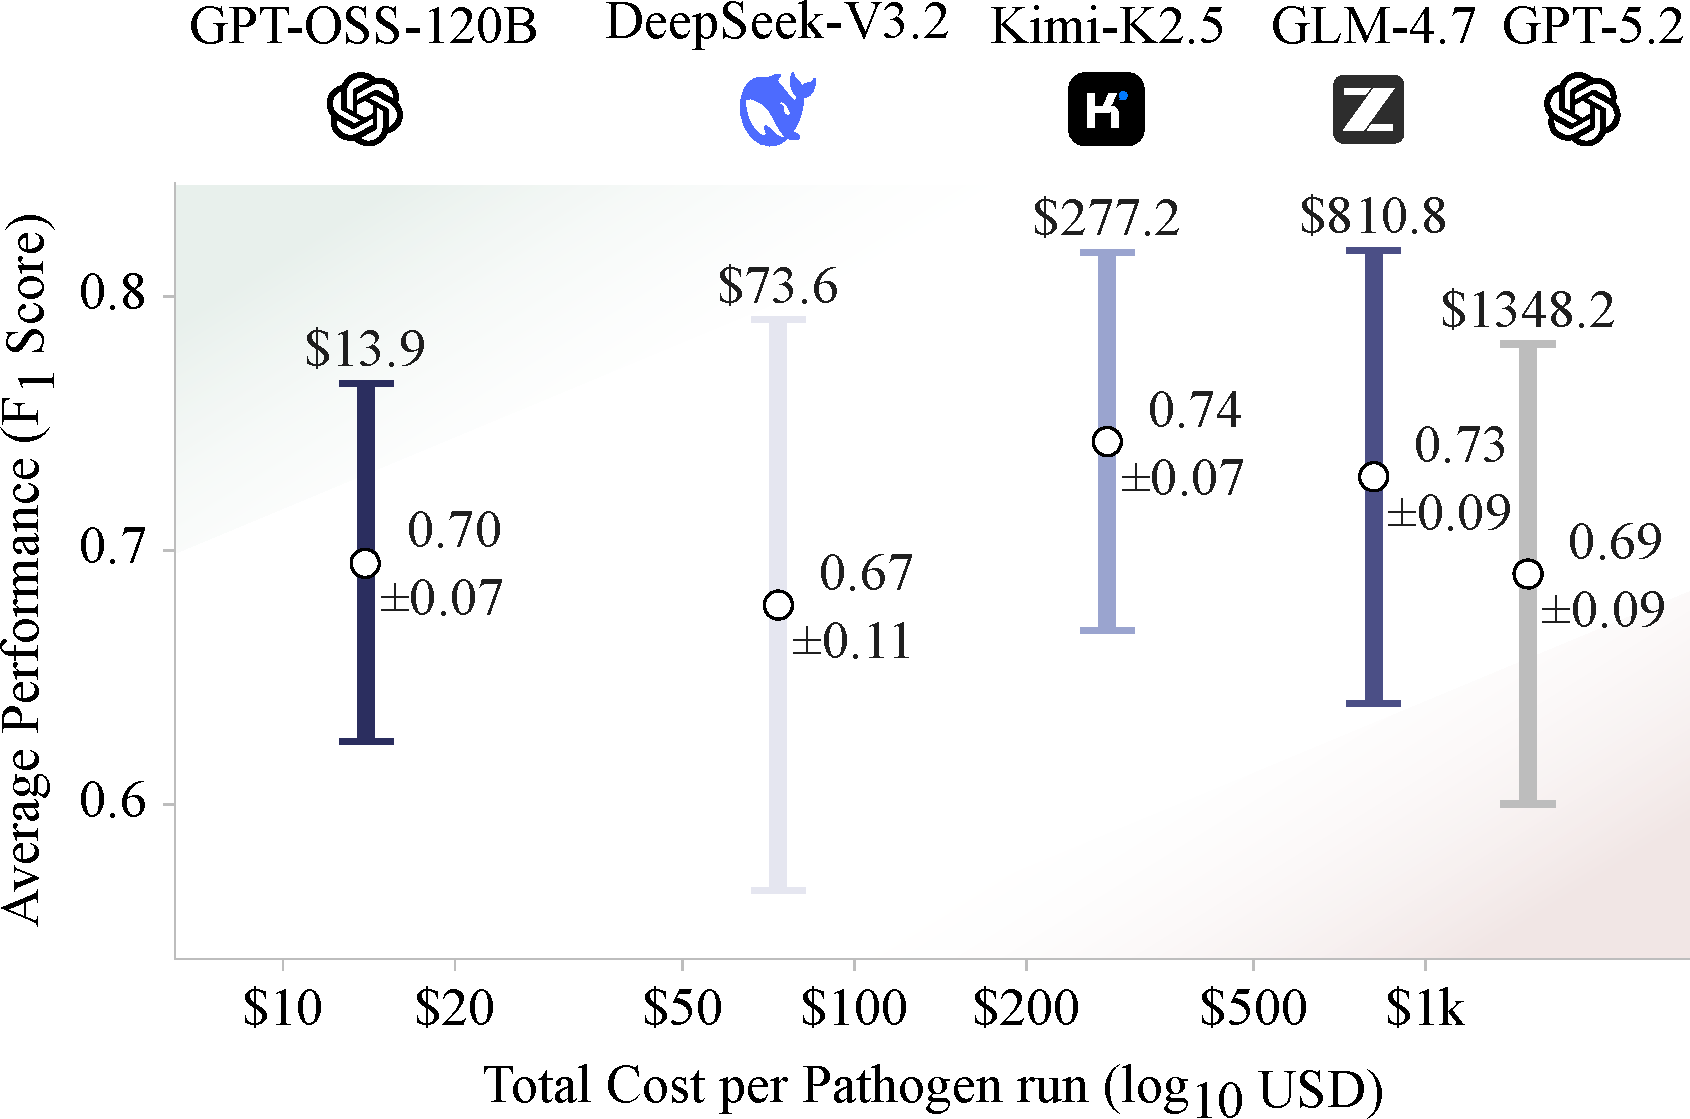
\includegraphics[width=\linewidth]{figures/ablation/cost_vs_accuracy_edited.pdf}
    \caption{\textbf{Comparing total cost against average performance for an \name{} pathogen run.} Each point shows a model's average macro $F_1$ across all \name{} pipeline stages plotted against its estimated total cost per pathogen run (USD, $\log_{10}$ scale), with vertical bars indicating one standard deviation in $F_1$ across stages. Costs are estimated from mean per-article token usage across a funnel of $9{,}132$ articles at abstract screening down to $395$ at data extraction (see \cref{fig:time_comparison} counts), multiplied by OpenRouter and OpenAI API pricing; full details in \cref{app:pipeline_statistics_costs}. We find that higher cost does not consistently correspond to higher performance.}
    \label{fig:cost_vs_performance}
\end{figure}


Consistent with \cref{tab:data_extraction_metrics}, models find the successive data extraction sub-tasks progressively harder: Flagging typically outperforms both Counts and Extraction. Outbreaks remain the exception to this trend, consistently across models, with precision notably lower for Flagging. Outbreak events are typically reported once but repeated across many papers as disease background. Across all extraction stages, the gap between the best and worst performing models is also considerably narrower than in the screening stages, suggesting that tool use during extraction may offset differences in base model capabilities.

\label{sec:cost_performance}


We further contextualise the model ablations by cost\footnote{All costs reported are in USD at the time of our experiment.} and aggregated performance across the full \name{} pipeline (\cref{fig:cost_vs_performance}). Higher cost and larger models do not consistently yield higher performance. \texttt{gpt-oss-120b} achieves competitive average performance ($F_1 = 0.70$) at the lowest total cost (\$13.9), over $96$ times cheaper than \texttt{GPT-5.2} (\$1,348). Despite being OpenAI's flagship closed-source model, \texttt{GPT-5.2} yields a lower average $F_1$ of $0.69$. More broadly, the best-performing model, \texttt{Kimi-K2.5} ($F_1 = 0.74$), sits in the mid-cost range (\$277), while \texttt{GLM-4.7} incurs the second-highest cost (\$811) for a comparable average $F_1$ of $0.73$. Variance across stages is also non-trivial for all models (ranging from $\pm 0.07$ to $\pm 0.11$), reflecting the uneven difficulty of pipeline stages as discussed above.

The substantial cost differences across models stem primarily from divergent per-article token usage, particularly at the parameter extraction stage. For example, \texttt{GPT-5.2} produces \num{91.1}K output tokens per article compared to \texttt{DeepSeek-V3.2}'s \num{3.0}K. Parameter extraction dominates overall compute; full per-stage token and cost breakdowns are reported in \cref{app:pipeline_statistics_costs} (Table~\ref{tab:token_usage_by_stage} and Figure~\ref{fig:tokens_costs_articles_split}). Taken together with the stage-level capability differences observed in \cref{sec:model_ablations}, these results suggest that the choice of LRM for \name{} involves a nuanced cost-performance trade-off, with no single model uniformly dominating across both dimensions.

